\documentclass[10pt,a4paper]{article}
\usepackage[utf8]{inputenc}
\usepackage{amsmath}
\usepackage{amsfonts}
\usepackage{amssymb}
\usepackage{graphicx}
\usepackage{verbatim}

\title{Parallel Computing Exercise 1}
\date{}
\author{Torsten Thoben, Marc Kassubeck}

\begin{document}

\maketitle

\section{Task 1 - Runtime influencing factors}
\begin{itemize}
\item Algorithmic complexity of the program (notation: $O(g(n))$, or $\Theta(g(n))$)(high):\\
This is a very high factor for program runtime as this is an estimation of the 'number of steps' that the algorithm has to make in order to produce the output. The importance of algorithmic complexity can be seen by the fact that one of the famous 'Millenium Problems' is indeed the question if $P=NP$.

\item Input size for the algorithm (the $n$ in $O(g(n))$)(high):\\
Also a very important factor. For example if you want to solve a partial differential equation on a regular grid it will cost more time and memory if you have 10, 10000 or $10^9$ grid points.

\item Underlying hardware (meaning number of transistors of CPU/GPU, clock rates, bus clock, etc.)(normal):\\
Better hardware has made previously infeasible problems solvable for even moderately priced consumer hardware in recent years. Thus the demand for better runtime can be approached by consecutively better hardware, but a less complex algorithm or a different approach to the problem (see points 1 and 2) can have considerably better effects. There are even problems (like integer factorization for moderately large integers of say 500 decimal digits) for which there is no computer and known algorithm in existence, which can solve this problem in practical time. So better hardware can simplify many practical problems but some problems are so inherently difficult that probably no computer will calculate a solution to those in a practical span of time.

\item Program language (low):\\
The use of a specific program language can have (even noticeable) impact on the run time of a program. Overhead like garbage collection or interpreting the code can slow down the execution of the program considerably, but neither does change the algorithmic complexity or the underlying hardware, so a change from a 'slow' to a 'fast' language doesn't have as much effect as changing one of the above points. 

\end{itemize}

\section{Task 2 - Runtime analysis}
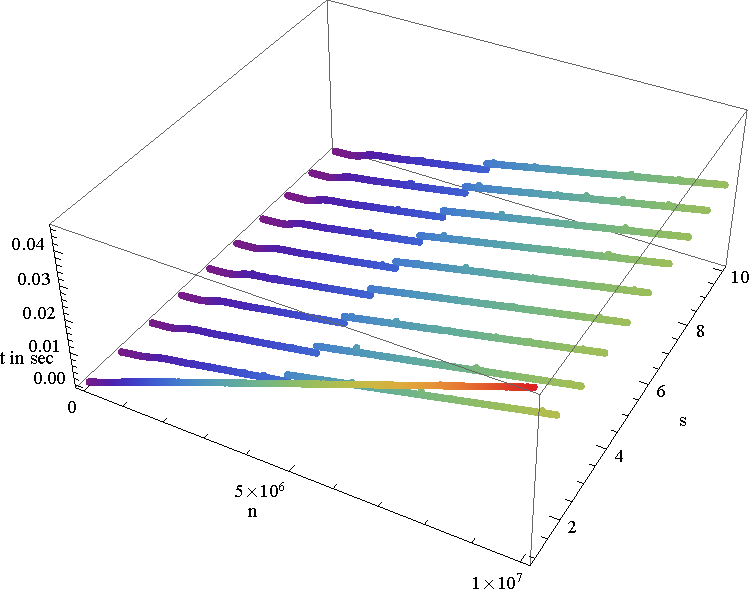
\includegraphics[scale=0.5]{graph1.pdf}
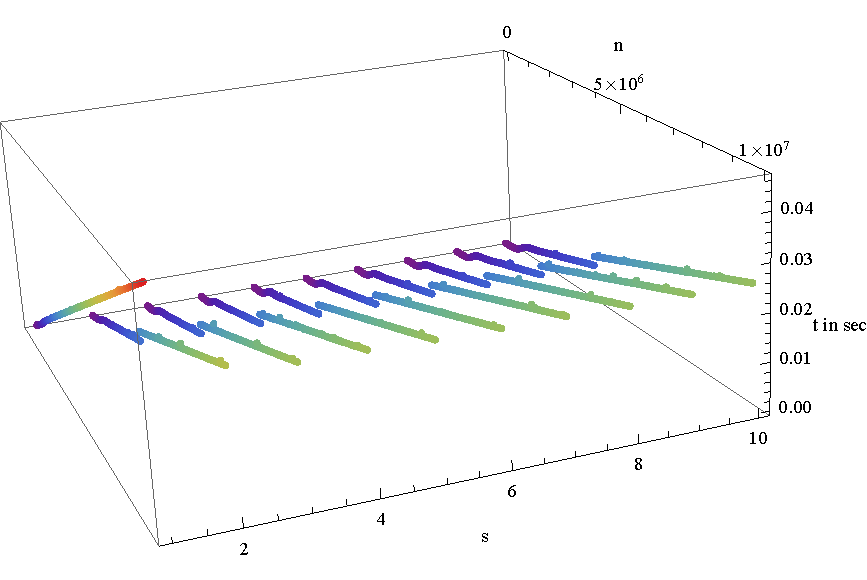
\includegraphics[scale=0.5]{graph2.pdf}

As expected the runtime increases approximately linear in $n$.\\
Surprisingly though, increasing $s$ decreases the runtime only at the transition $s=1 \rightarrow s=2$ and stays constant for constant $n$.

\section{Task 3 - Roundtrip time}

\subsection{1 Node, 2 Processors per Node}
\verbatiminput{task3.out}

\subsection{2 Nodes, 1 Processor per Node}
\verbatiminput{task3_remote.out}

\subsection{Analysis}
As can be clearly seen the latency with 2 nodes and 1 processor per node is much higher than with 1 node and 2 processors per node (factor $\frac{0.012855s}{0.001747s}=7.3583285$).\\
This can be expected as in the latter case both Processors are probably physical cores on one chip, whereas in the first case the program is executed on physically separated machines, which are connected via some kind of network connection. The higher latency can therefore be expected, keeping the physical distances of the memory of these 2 methods of invocation in mind.

\end{document}